\section{Bidirectional Search} 
\label{ch:bs}

Bidirectional search simultaneously searches from the start state to the goal state (\textbf{forward searching}) and from the goal state to the start state  (\textbf{backward searching}) hoping that these two searches will meet. The time and space complexity was reduced from $O(b^d)$ to $O(2 * b^{d/2}) = O(b^{d/2}) << O(b^d)$, where $b$ is the branching factor and $d$ is the depth of the shallowest solution.

\subsection{Implementation}


The algorithm uses the \textbf{Breadth-First Search policy}, meaning that it takes the shallowest node first. It stops when the forward and backward search intersect. If no solutions is found, than it returns \textit{None}.

We used two sets one representing the explored nodes that are still in the queue and another one, that contains the visited nodes that were popped out of the queue.
Entering the while loop, we firstly analyze the forward search. Take the next node from the corresponding queue and if it is not yet visited we put it in the visited set. After we have iterated through the nodes of the backward search, if there is a meeting point then we return the current path and the path accumulated by the backward search in reverse order.

Next we analyze the backward search the same way as we did for the forward search, the only difference being that we replace each action with its opposite action, we reverse the list containing them and add it to the accumulated path.

The motivation behind using sets is that they are more efficient than lists in verifying whether they contain an arbitrary element.

Source code: Appendix \ref{sec:code_bs}.

\begin{figure}[ht]
    \centering
    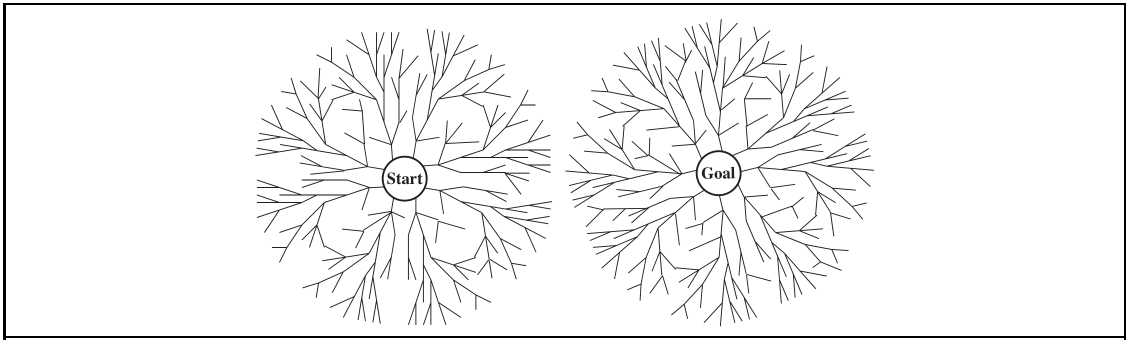
\includegraphics[width=.8\linewidth]{fig/bs.png}
    \caption{Visualization of the bidirectional search algorithm. \cite{aima2020}} 
    \label{fig:bs}
\end{figure}

